\section{Evaluation}


The original goal of the project is to create a scalable logging algorithm that does not act as a bottleneck for the database as a whole. The data shown below was collected to determine the scalability of the algorithm. 

Four algorithms were tested to generate these results. The first is a generic serial logging algorithm, the second is a serial logging algorithm with certain optimizations put in place, the third is the batch logging algorithm, and the last is a parallel logging algorithm. These different aAll of these are explained in further detail earlier in this paper. \newline

The results shown indicate the amount of time one txn would take to log. The goal is to minimize the amount the time increases as the thread count increases, indicating high scalability and preventing logging from becoming a bottleneck. Each of the four algorithms was tested on a maximum of 10000 txns and buffer sizes ranging from 10 to 100. 10 tests were run for each buffer size, and the average of these 10 test are shown below. \newline 

NOTE: MAKE ALL OF THESE TABLES
\begin{table}[h!]
  \centering
  \caption{Serial logging, without optimization, four threads Results}
  \label{tab:table1}
  \begin{tabular}{l|c|r}
    Buffer size & Average log time per txn & Number of txns\\
    \hline
    10 &  7.98827246297e-06 & 3981.4\\
    \hline
    20 &  7.09085828262e-06 & 35842.6\\
    \hline
    30 & 1.00192992279e-05 & 43720.9\\
    \hline
    40 & 1.43699414518e-05 & 43297.9\\
    \hline
    50 &  1.33267980447e-05 & 43549.2\\
    \hline
    60 &  1.1985913315e-05 & 43616.3\\
    \hline
    70 &  1.14592003908e-05  & 43672.7\\
    \hline
    80 &  1.10223567894e-05 & 43504.3\\
    \hline
    90 &  9.95585073659e-06 & 39617.3\\
    \hline
    100 &  9.77583551714e-06  & 39512.7\\
  \end{tabular}
\end{table}
Results for serial logging without optimization on standard four threads:
Average log time per txn for buffer_size 10: 7.98827246297e-06 with 39831.4 txns.
Average log time per txn for buffer_size 20: 7.09085828262e-06 with 35842.6 txns.
Average log time per txn for buffer_size 30: 1.00192992279e-05 with 43720.9 txns.
Average log time per txn for buffer_size 40: 1.43699414518e-05 with 43297.9 txns.
Average log time per txn for buffer_size 50: 1.33267980447e-05 with 43549.2 txns.
Average log time per txn for buffer_size 60: 1.1985913315e-05 with 43616.3 txns.
Average log time per txn for buffer_size 70: 1.14592003908e-05 with 43672.7 txns.
Average log time per txn for buffer_size 80: 1.10223567894e-05 with 43504.3 txns.
Average log time per txn for buffer_size 90: 9.95585073659e-06 with 39617.3 txns.
Average log time per txn for buffer_size 100: 9.77583551714e-06 with 39512.7 txns.


Results for serial logging with opimization on standard four threads:


Average log time per txn for buffer_size 10: 8.4024601054e-06 with 39814.7 txns.
Average log time per txn for buffer_size 20: 7.94581075305e-06 with 35738.3 txns.
Average log time per txn for buffer_size 30: 8.29208836395e-06 with 43826.1 txns.
Average log time per txn for buffer_size 40: 1.21009485441e-05 with 43709.4 txns.
Average log time per txn for buffer_size 50: 1.15426346849e-05 with 43542.6 txns.
Average log time per txn for buffer_size 60: 1.06209155302e-05 with 43513.1 txns.
Average log time per txn for buffer_size 70: 1.08573198778e-05 with 43391.0 txns.
Average log time per txn for buffer_size 80: 9.5191373736e-06 with 43707.1 txns.
Average log time per txn for buffer_size 90: 8.75585618379e-06 with 39517.5 txns.
Average log time per txn for buffer_size 100: 8.08590952704e-06 with 39549.7 txns.

Results for serial logging without opimization on eight threads:


Average log time per txn for buffer_size 10: 4.04340885057e-05 with 78395.9 txns.
Average log time per txn for buffer_size 20: 5.88612024086e-05 with 68059.7 txns.
Average log time per txn for buffer_size 30: 6.87869859705e-05 with 82370.1 txns.
Average log time per txn for buffer_size 40: 6.1601780077e-05 with 83024.6 txns.
Average log time per txn for buffer_size 50: 5.49539990923e-05 with 81959.7 txns.
Average log time per txn for buffer_size 60: 4.52139548576e-05 with 84458.9 txns.
Average log time per txn for buffer_size 70: 4.02535824733e-05 with 83681.0 txns.
Average log time per txn for buffer_size 80: 3.71636342753e-05 with 83818.1 txns.
Average log time per txn for buffer_size 90: 2.91596069681e-05 with 76400.8 txns.
Average log time per txn for buffer_size 100: 2.5959065368e-05 with 77982.6 txns.

Results for serial logging with opimization on eight threads:


Average log time per txn for buffer_size 10: 7.2372970539e-05 with 77455.7 txns.
Average log time per txn for buffer_size 20: 5.06991711113e-05 with 69759.8 txns.
Average log time per txn for buffer_size 30: 5.21307230369e-05 with 84272.5 txns.
Average log time per txn for buffer_size 40: 4.68441761639e-05 with 84701.5 txns.
Average log time per txn for buffer_size 50: 4.07150340118e-05 with 85251.5 txns.
Average log time per txn for buffer_size 60: 3.74521773965e-05 with 85051.3 txns.
Average log time per txn for buffer_size 70: 3.39602513669e-05 with 85401.2 txns.
Average log time per txn for buffer_size 80: 3.17901883362e-05 with 85266.8 txns.
Average log time per txn for buffer_size 90: 2.67467697626e-05 with 77169.7 txns.
Average log time per txn for buffer_size 100: 2.60182905193e-05 with 77739.4 txns.


%BATCH LOGGING RESULTS
We tested various implementations of batch logging with a varying number of loggers. The average total run time and average time spent logging were recorded and graphed. Since we want to reduce run and logging times, lower is better. We expected an increase in the number of loggers to correspond with faster run and logging times, and the results back that hypothesis.
\begin{figure}
	\caption{Batch Logging Results}
	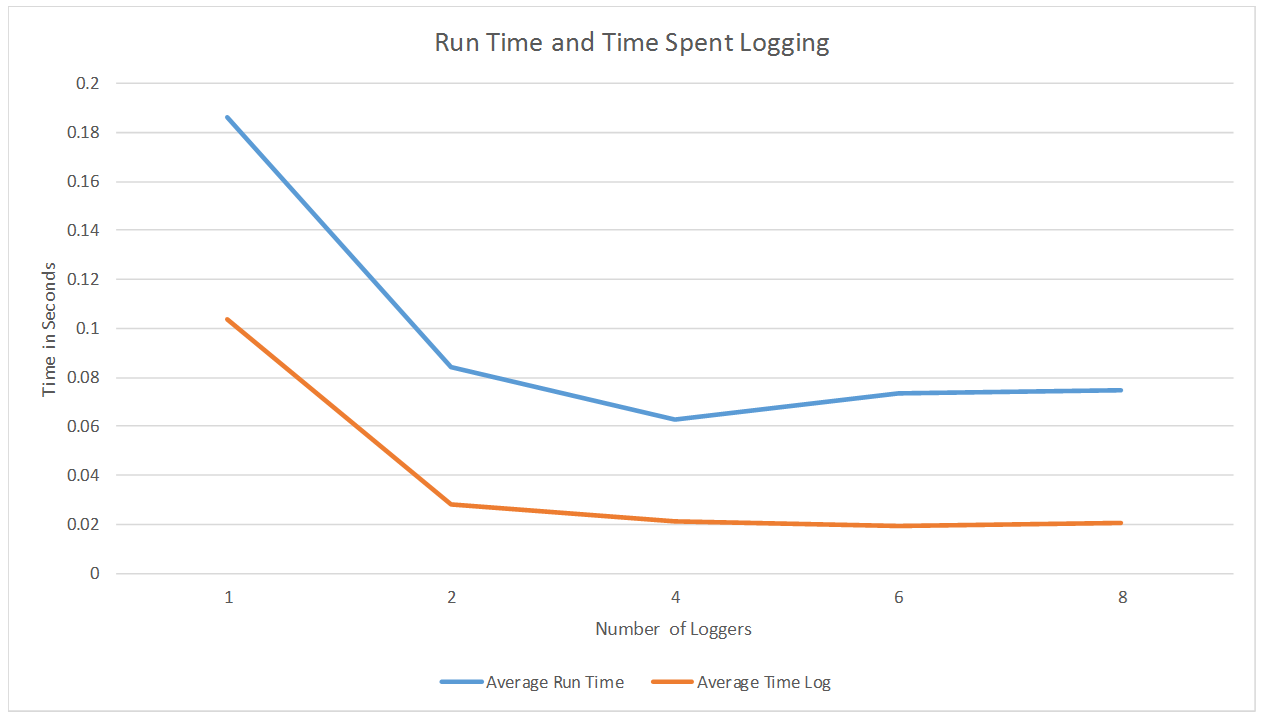
\includegraphics[width=\textwidth]{BatchLoggingResults.png}
\end{figure}